\chapter{Results}

\section{Results Overview and Reporting Conventions}

This chapter reports the empirical outcomes from the 44 authoritative configurations defined in Chapter~3: 32 core configurations and 12 sensitivity configurations. The remaining committed run directories---25 development or validation runs and 17 invalid, incomplete, duplicated or superseded runs---do not contribute to the results reported here. Functional correctness is expressed as both the number of tasks solved and the corresponding problem-level pass@1. Here, pass@1 denotes the strategy-level task success proportion under the frozen protocol: Single-pass requires its sole candidate to pass, Best-of-5 requires any of its five candidates to pass, adaptive refinement requires any candidate in its trajectory to pass, and fixed-$k=5$ uses ever-solved as its principal discovery outcome. For fixed-$k=5$ refinement, the principal discovery outcome is whether a task was solved at any iteration; correctness at iteration five is reported separately as a stability diagnostic.

The primary Qwen2.5-Coder-7B-Instruct configuration used non-quantised bfloat16 inference through Hugging Face/CUDA. The replication configuration used CodeLlama-13B-Instruct with bitsandbytes 8-bit loading through Hugging Face/CUDA. Differences between these configurations are therefore reported as cross-configuration observations. They do not isolate model family, parameter scale or numerical representation.

Best-of-5 and refinement were generation-budget-matched in the sense that each permitted at most five generations per task. Their realised computation was not identical: Best-of-5 always generated five independent candidates at temperature 0.8 using seeds 42--46, whereas adaptive refinement used temperature 0.2, seed 42 within each trajectory and could terminate before its fifth generation. Their comparison consequently evaluates two complete inference policies rather than the isolated causal effect of execution feedback under identical decoding settings. Model calls are used as the principal main-text efficiency measure; they count generation requests and are not treated as equivalent to floating-point operations, latency or energy use.

\section{Standard-Benchmark Functional Correctness}

Table~\ref{tab:standard-results} presents the standard-benchmark results, while Figure~\ref{fig:standard-pass} shows the corresponding pass@1 values. Fixed-$k=5$ is omitted from this headline table and figure because its ever-solved outcome was identical to adaptive refinement in every standard condition; that ablation is examined separately in Section~4.6.

\begin{table}[htbp]
    \centering
    \caption{Functional correctness and model calls on the standard benchmarks. Percentages are problem-level pass@1; counts in parentheses are solved tasks.}
    \label{tab:standard-results}
    \scriptsize
    \renewcommand{\arraystretch}{1.15}
    \resizebox{\textwidth}{!}{%
    \begin{tabular}{llrrrrr}
        \hline
        Model configuration & Benchmark & Single-pass & Best-of-5 & Adaptive & Adaptive calls & BO5 calls \\
        \hline
        Qwen bfloat16 & HumanEval & 86.59\% (142/164) & 92.68\% (152/164) & 90.24\% (148/164) & 199 & 820 \\
        Qwen bfloat16 & Sanitised MBPP & 71.90\% (307/427) & 78.92\% (337/427) & 82.44\% (352/427) & 647 & 2,135 \\
        CodeLlama 8-bit & HumanEval & 41.46\% (68/164) & 62.20\% (102/164) & 53.05\% (87/164) & 311 & 820 \\
        CodeLlama 8-bit & Sanitised MBPP & 44.96\% (192/427) & 61.59\% (263/427) & 60.19\% (257/427) & 821 & 2,135 \\
        \hline
    \end{tabular}}
\end{table}

\begin{figure}[htbp]
    \centering
    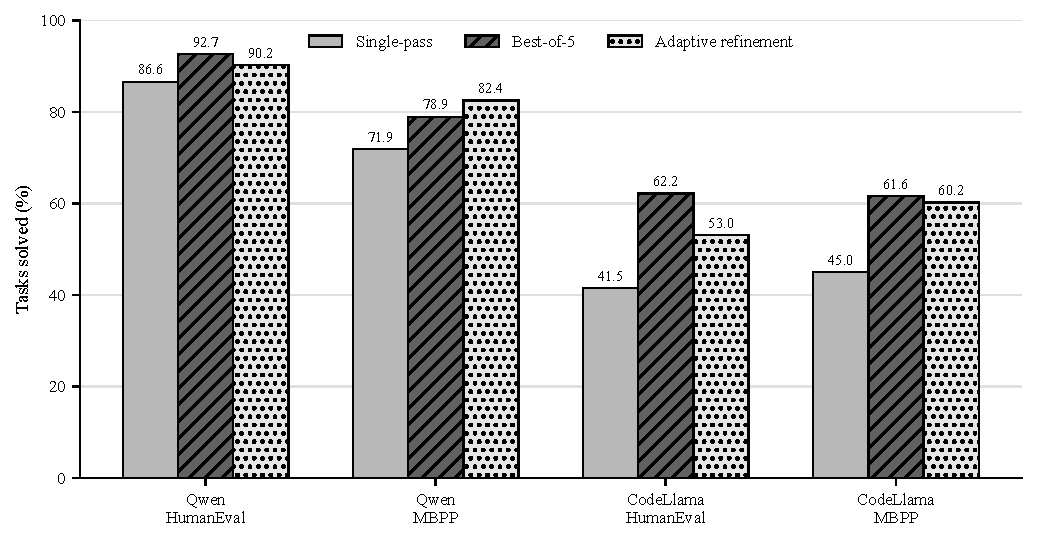
\includegraphics[width=\textwidth]{figures/figure_4_1_standard_pass_at_1.pdf}
    \caption{Problem-level pass@1 for the three principal discovery policies on HumanEval and sanitised MBPP. Qwen denotes non-quantised bfloat16 inference and CodeLlama denotes bitsandbytes 8-bit inference.}
    \label{fig:standard-pass}
\end{figure}

\subsection{Qwen Results}

On HumanEval, Qwen single-pass generation solved 142 of 164 tasks (86.59\%). Best-of-5 increased this to 152 tasks (92.68\%), the highest result in this condition. Adaptive refinement solved 148 tasks (90.24\%): six more than single-pass, but four fewer than Best-of-5. It reached this outcome with 199 model calls, compared with 164 for single-pass and 820 for Best-of-5.

The Qwen ranking changed on sanitised MBPP. Single-pass solved 307 of 427 tasks (71.90\%) and Best-of-5 solved 337 (78.92\%). Adaptive refinement solved 352 tasks (82.44\%), improving on single-pass by 45 tasks and on Best-of-5 by 15. The adaptive procedure used 647 calls, compared with 2,135 for Best-of-5. Thus Qwen adaptive refinement was the highest-scoring of the three policies on sanitised MBPP, whereas Best-of-5 remained highest on HumanEval.

\subsection{CodeLlama Replication}

For CodeLlama on HumanEval, single-pass solved 68 of 164 tasks (41.46\%), Best-of-5 solved 102 (62.20\%), and adaptive refinement solved 87 (53.05\%). Refinement therefore recovered 19 additional tasks relative to single-pass but remained 15 tasks below Best-of-5. Adaptive refinement used 311 calls rather than Best-of-5's 820.

On sanitised MBPP, CodeLlama single-pass solved 192 of 427 tasks (44.96\%). Best-of-5 solved 263 (61.59\%), while adaptive refinement solved 257 (60.19\%). The six-task numerical deficit for adaptive refinement was substantially smaller than its 15-task HumanEval deficit. Adaptive refinement used 821 calls, 1,314 fewer than Best-of-5. This MBPP outcome did not reproduce the Qwen result in which refinement exceeded Best-of-5, but it did reproduce improvement over single-pass and a lower realised call count than five independent samples.

\subsection{Cross-Configuration Pattern}

Across both evaluated configurations and both standard benchmarks, adaptive refinement improved on single-pass: by 3.66 and 10.54 percentage points for Qwen on HumanEval and MBPP, and by 11.59 and 15.22 points for CodeLlama. Its ranking relative to Best-of-5 was not uniform. It trailed Best-of-5 in three conditions and led in Qwen sanitised MBPP. Figure~\ref{fig:standard-pass} also shows that the absolute pass@1 levels differed substantially between model configurations. Since model identity, parameter scale and numerical representation vary together, these absolute differences are descriptive and are not attributed to a single factor.

\section{Adaptive Refinement versus Best-of-5}

\subsection{Standard-Benchmark Paired Comparisons}

The aggregate differences were evaluated using the pre-specified exact conditional two-sided McNemar test. The direction of every effect below is adaptive refinement minus Best-of-5; $p$-values are unadjusted and no continuity correction was applied.

For Qwen HumanEval, three tasks were solved only by adaptive refinement and seven only by Best-of-5. The paired risk difference was $-2.44$ percentage points, the matched odds ratio was 0.4286, and the difference was not statistically significant ($p=0.34375$). On Qwen sanitised MBPP, 33 tasks were adaptive-only and 18 were Best-of-5-only. The risk difference was $+3.51$ points and the matched odds ratio was 1.8333; the exact condition-specific test crossed the pre-specified threshold ($p=0.048873892$). The small margin relative to $\alpha=0.05$, its unadjusted status and the observed 15-task effect are all retained rather than reducing the result to a binary significance label.

For CodeLlama HumanEval, six tasks were adaptive-only and 21 were Best-of-5-only. The risk difference was $-9.15$ percentage points, with the direction favouring Best-of-5. It was statistically significant (matched odds ratio 0.2857; $p=0.005924612$). For CodeLlama sanitised MBPP, the discordant cells were 29 adaptive-only and 35 Best-of-5-only. The risk difference was $-1.41$ points and was not statistically significant (matched odds ratio 0.8286; $p=0.532308776$). The paired evidence therefore distinguishes the sizeable CodeLlama HumanEval deficit from the smaller and statistically unresolved MBPP difference.

\subsection{Generation-Budget Comparison}

The paired results establish that the relative ranking depended on the evaluated model--benchmark condition. They do not establish that feedback alone produced the differences. Best-of-5 combined five independent seeds with temperature 0.8, whereas refinement used a dependent revision trajectory at temperature 0.2. Accordingly, the positive Qwen MBPP result is evidence that the complete adaptive execution-feedback policy outperformed the complete Best-of-5 policy in that condition; it is not an estimate of feedback's isolated causal contribution under identical sampling.

The comparison nevertheless answers the practical generation-budget question posed by the experimental design. On HumanEval, Best-of-5 converted its five-generation allowance into the highest pass@1 for both model configurations. On sanitised MBPP, adaptive refinement used fewer realised calls and either exceeded Best-of-5 for Qwen or remained within six tasks for CodeLlama. Figure~\ref{fig:accuracy-calls} makes this accuracy--call relationship explicit without treating calls as interchangeable across model configurations.

\begin{figure}[htbp]
    \centering
    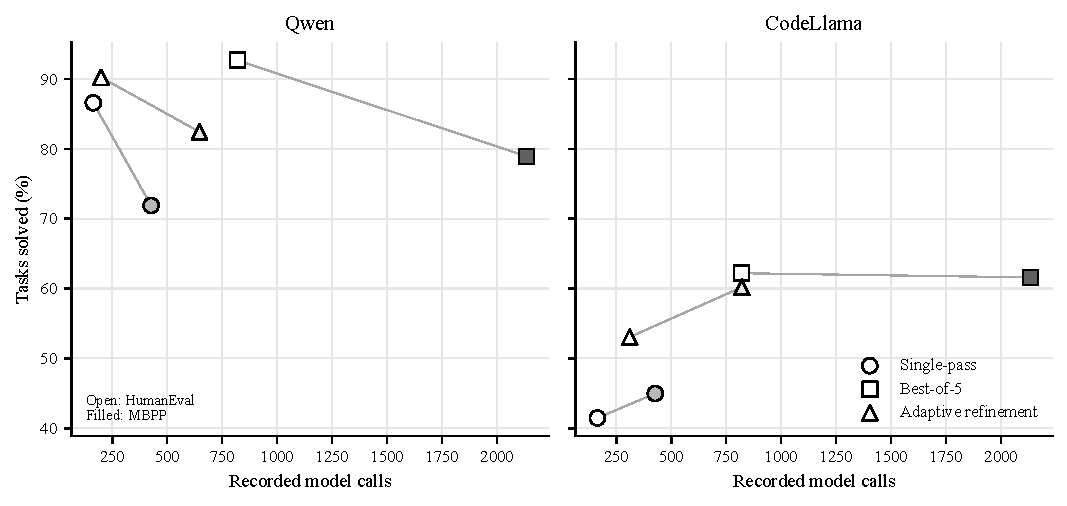
\includegraphics[width=\textwidth]{figures/figure_4_2_accuracy_calls.pdf}
    \caption{Standard-benchmark functional correctness against recorded model calls. Lines connect different benchmarks for visual identification only; they do not represent trajectories or equivalence of per-call computational cost across configurations.}
    \label{fig:accuracy-calls}
\end{figure}

\section{Harder Pro-Benchmark Results}

Table~\ref{tab:pro-results} and Figure~\ref{fig:pro-pass} report the corresponding results on HumanEval Pro and MBPP Pro. Best-of-5 attained the highest pass@1 in all four Pro conditions. Frozen 10,000-resample problem-level percentile bootstrap intervals are reported below for Best-of-5 and adaptive refinement; the paired McNemar tests remain the formal comparisons because the observations are matched by task.

\begin{table}[htbp]
    \centering
    \caption{Functional correctness, calls and adaptive-versus-Best-of-5 exact McNemar results on the Pro benchmarks.}
    \label{tab:pro-results}
    \scriptsize
    \renewcommand{\arraystretch}{1.15}
    \resizebox{\textwidth}{!}{%
    \begin{tabular}{llrrrrrr}
        \hline
        Model configuration & Benchmark & Single-pass & Best-of-5 & Adaptive & Adaptive calls & BO5 calls & Exact $p$ \\
        \hline
        Qwen bfloat16 & HumanEval Pro & 65.24\% (107/164) & 78.66\% (129/164) & 70.12\% (115/164) & 256 & 820 & 0.00257683 \\
        Qwen bfloat16 & MBPP Pro & 60.32\% (228/378) & 76.46\% (289/378) & 67.99\% (257/378) & 620 & 1,890 & $5.6141\!\times\!10^{-6}$ \\
        CodeLlama 8-bit & HumanEval Pro & 28.66\% (47/164) & 43.29\% (71/164) & 33.54\% (55/164) & 340 & 820 & 0.00700037 \\
        CodeLlama 8-bit & MBPP Pro & 37.83\% (143/378) & 54.50\% (206/378) & 46.30\% (175/378) & 718 & 1,890 & 0.000244397 \\
        \hline
    \end{tabular}}
\end{table}

\begin{figure}[htbp]
    \centering
    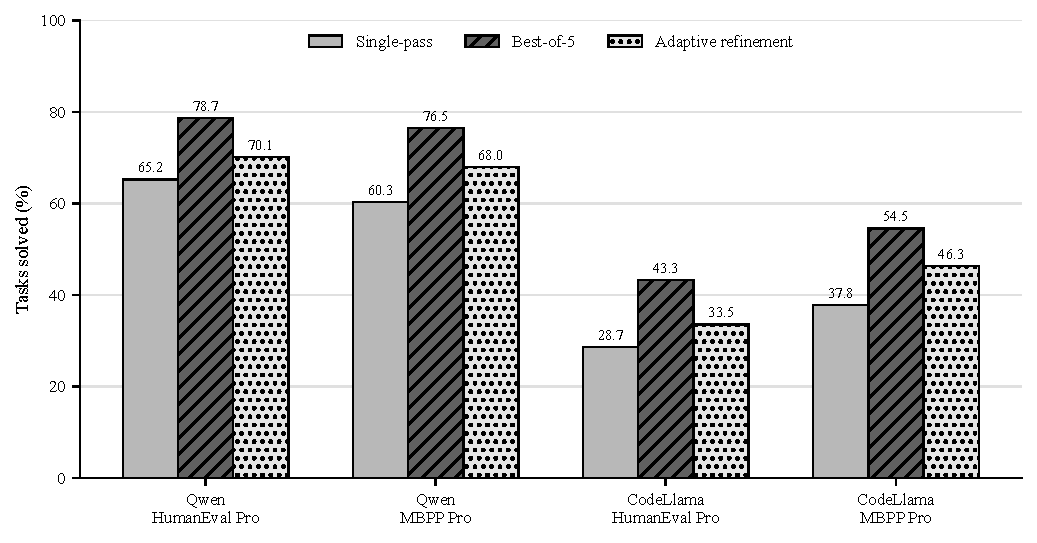
\includegraphics[width=\textwidth]{figures/figure_4_3_pro_pass_at_1.pdf}
    \caption{Problem-level pass@1 on HumanEval Pro and MBPP Pro. Best-of-5 was highest in each evaluated model--benchmark condition.}
    \label{fig:pro-pass}
\end{figure}

\subsection{HumanEval Pro}

For Qwen, single-pass solved 107 of 164 HumanEval Pro tasks (65.24\%). Best-of-5 solved 129 (78.66\%) and adaptive refinement solved 115 (70.12\%). Their bootstrap 95\% intervals were [72.56\%, 84.76\%] and [62.80\%, 76.83\%], respectively. Three tasks were adaptive-only and 17 were Best-of-5-only, giving a risk difference of $-8.54$ points, matched odds ratio 0.1765 and $p=0.00257683$.

For CodeLlama, single-pass solved 47 HumanEval Pro tasks (28.66\%). Best-of-5 solved 71 (43.29\%) and adaptive refinement solved 55 (33.54\%). Their bootstrap intervals were [35.98\%, 50.61\%] and [26.22\%, 40.85\%], respectively. The discordant counts were eight adaptive-only and 24 Best-of-5-only. The risk difference was $-9.76$ points and was statistically significant (matched odds ratio 0.3333; $p=0.00700037$).

\subsection{MBPP Pro}

For Qwen on MBPP Pro, single-pass solved 228 tasks (60.32\%). Best-of-5 solved 289 (76.46\%) and adaptive refinement solved 257 (67.99\%). Their bootstrap intervals were [72.22\%, 80.69\%] and [63.23\%, 72.75\%], respectively. Nine tasks were adaptive-only and 41 were Best-of-5-only; the risk difference was $-8.47$ points, the matched odds ratio was 0.2195, and $p=5.6141\times10^{-6}$.

CodeLlama single-pass solved 143 MBPP Pro tasks (37.83\%), Best-of-5 solved 206 (54.50\%), and adaptive refinement solved 175 (46.30\%). The Best-of-5 bootstrap interval was [49.47\%, 59.79\%], while the adaptive interval was [41.53\%, 51.32\%]. Nineteen tasks were adaptive-only and 50 were Best-of-5-only, producing a $-8.20$-point risk difference, matched odds ratio 0.3800 and $p=0.000244397$.

\subsection{Cross-Configuration Pattern on Harder Tasks}

Adaptive refinement improved over single-pass in all four Pro conditions, by between 4.88 and 8.47 percentage points. Unlike the standard benchmarks, however, it did not rank first in any Pro condition. Its deficit relative to Best-of-5 was similar across the four paired comparisons, ranging from 8.20 to 9.76 points, and each difference was statistically significant under the unadjusted condition-specific test. This common ranking occurred despite substantial differences in absolute pass@1 between the two model configurations and between the benchmark variants.

The Pro evidence therefore changes the observed strategy ranking relative to Qwen sanitised MBPP, where adaptive refinement was highest. It does not eliminate the refinement gain over a single generation: Qwen gained eight HumanEval Pro and 29 MBPP Pro tasks, while CodeLlama gained eight and 32 respectively. Rather, the five independent Best-of-5 candidates discovered more solutions than the adaptive trajectory within the same maximum generation allowance on all four harder conditions.

\section{Computational Efficiency}

Adaptive refinement used fewer model calls than Best-of-5 in every standard and Pro condition. On the standard benchmarks, calls fell from 820 to 199 for Qwen HumanEval, a reduction of 621 calls (75.7\%); from 2,135 to 647 for Qwen sanitised MBPP, a reduction of 1,488 (69.7\%); from 820 to 311 for CodeLlama HumanEval, a reduction of 509 (62.1\%); and from 2,135 to 821 for CodeLlama sanitised MBPP, a reduction of 1,314 (61.5\%). These reductions reflect adaptive termination rather than an equal realised generation count.

The same pattern held on the Pro benchmarks. Qwen adaptive refinement used 256 rather than 820 calls on HumanEval Pro (68.8\% fewer) and 620 rather than 1,890 on MBPP Pro (67.2\% fewer). CodeLlama used 340 rather than 820 calls on HumanEval Pro (58.5\% fewer) and 718 rather than 1,890 on MBPP Pro (62.0\% fewer). The call reductions therefore ranged from 58.5\% to 75.7\% across the eight authoritative conditions.

The accuracy consequence of those reductions differed by condition. Qwen sanitised MBPP combined fewer calls with a higher pass@1 than Best-of-5. CodeLlama sanitised MBPP combined 61.5\% fewer calls with a non-significant 1.41-point deficit. In contrast, both HumanEval conditions and all four Pro conditions showed lower adaptive pass@1, with the Pro deficits all statistically significant. Figure~\ref{fig:accuracy-calls} visualises the standard results, but does not imply that a Qwen call and a CodeLlama call have equal computational cost.

Authoritative prompt-token, completion-token and wall-clock totals were also recorded. They are not reproduced as a complete main-text matrix because their interpretation depends on prompt growth, generated length, model representation, hardware and run conditions. Model-call counts consequently provide a transparent measure of generation frequency, not a substitute for unmeasured FLOPs, energy or financial cost.

\section{Adaptive Convergence and Forced Continuation}

Table~\ref{tab:convergence-results} compares adaptive refinement with exactly five forced refinement iterations. Across all eight authoritative model--benchmark conditions, the adaptive and fixed procedures had identical ever-solved task sets. The paired discordant cells were therefore zero in both directions in every condition: the risk difference was zero, the Haldane--Anscombe-adjusted matched odds ratio was 1.0, and the exact McNemar $p$-value was 1.0. Forced continuation discovered no additional task beyond adaptive stopping.

\begin{table}[htbp]
    \centering
    \caption{Adaptive convergence and fixed-$k=5$ continuation. Regression denominators are fixed-run tasks solved at least once.}
    \label{tab:convergence-results}
    \scriptsize
    \renewcommand{\arraystretch}{1.15}
    \resizebox{\textwidth}{!}{%
    \begin{tabular}{llrrrrr}
        \hline
        Model configuration & Benchmark & Ever solved A/F & Fixed final & Adaptive calls & Fixed calls & Regressions \\
        \hline
        Qwen bfloat16 & HumanEval & 148/148 & 143 & 199 & 820 & 5/148 (3.4\%) \\
        Qwen bfloat16 & Sanitised MBPP & 352/352 & 334 & 647 & 2,135 & 18/352 (5.1\%) \\
        CodeLlama 8-bit & HumanEval & 87/87 & 78 & 311 & 820 & 9/87 (10.3\%) \\
        CodeLlama 8-bit & Sanitised MBPP & 257/257 & 211 & 821 & 2,135 & 46/257 (17.9\%) \\
        Qwen bfloat16 & HumanEval Pro & 115/115 & 114 & 256 & 820 & 1/115 (0.9\%) \\
        Qwen bfloat16 & MBPP Pro & 257/257 & 253 & 620 & 1,890 & 4/257 (1.6\%) \\
        CodeLlama 8-bit & HumanEval Pro & 55/55 & 54 & 340 & 820 & 1/55 (1.8\%) \\
        CodeLlama 8-bit & MBPP Pro & 175/175 & 164 & 718 & 1,890 & 11/175 (6.3\%) \\
        \hline
    \end{tabular}}
\end{table}

\begin{figure}[htbp]
    \centering
    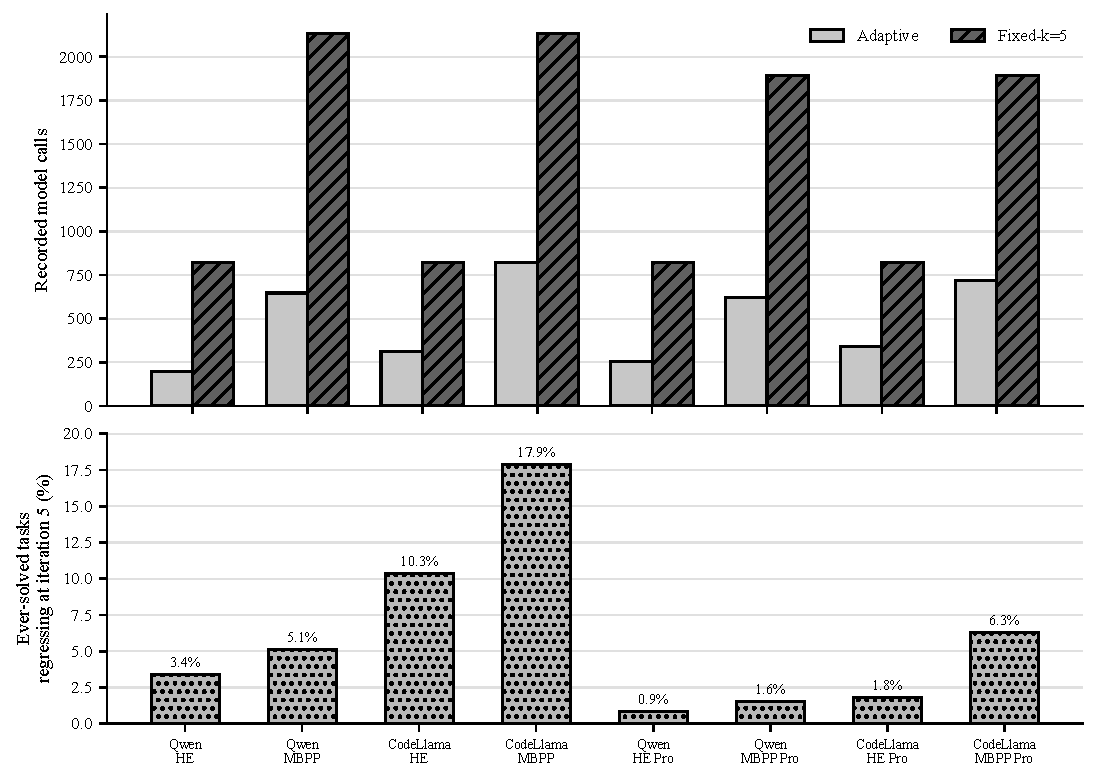
\includegraphics[width=\textwidth]{figures/figure_4_4_convergence_regressions.pdf}
    \caption{Recorded model calls under adaptive and fixed-$k=5$ refinement, with the proportion of fixed-run ever-solved tasks that failed at iteration five. A/F in Table~\ref{tab:convergence-results} denotes adaptive/fixed ever-solved counts.}
    \label{fig:convergence-regressions}
\end{figure}

The additional fixed calls were 621 and 1,488 for Qwen on the standard benchmarks, 509 and 1,314 for CodeLlama, 564 and 1,270 for Qwen on the Pro benchmarks, and 480 and 1,172 for CodeLlama. Although discovery outcomes were unchanged, final-iteration correctness decreased in every condition. The standard fixed runs regressed from ever-solved to final-failing on 5/148 Qwen HumanEval tasks (3.4\%), 18/352 Qwen MBPP tasks (5.1\%), 9/87 CodeLlama HumanEval tasks (10.3\%), and 46/257 CodeLlama MBPP tasks (17.9\%). The corresponding Pro rates were 0.9\%, 1.6\%, 1.8\% and 6.3\%.

The frozen trajectory audit identified a common recorded prompt pattern in the regression cases: after a successful execution reported ``All assertions passed.'', forced continuation nevertheless supplied a subsequent request for a corrected solution. This is reported as an observed association in the persisted trajectories. The results do not by themselves establish that this wording caused each later failure. Empirically, however, retaining the earlier passing candidate avoided the final-state losses while producing the same ever-solved outcome with fewer calls.

\section{Sensitivity Analysis}

The sensitivity analysis used the same fixed 100-task HumanEval subset for both model configurations. Figure~\ref{fig:sensitivity} presents the feedback-length and temperature results. These are fixed-seed descriptive comparisons; no frozen sensitivity confidence intervals or paired statistical outputs are available.

\begin{figure}[htbp]
    \centering
    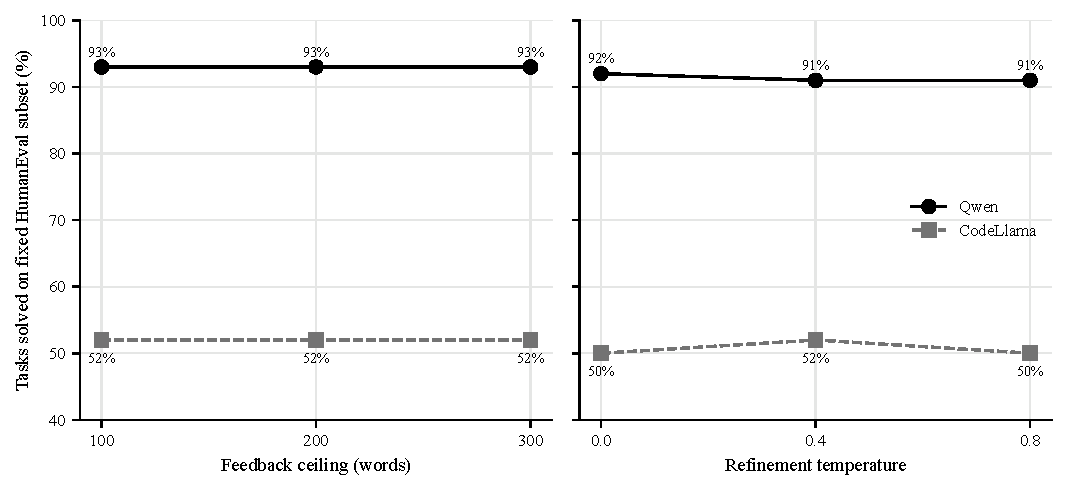
\includegraphics[width=\textwidth]{figures/figure_4_5_sensitivity.pdf}
    \caption{Adaptive-refinement sensitivity on the fixed 100-task HumanEval subset. The left panel varies the feedback ceiling at temperature 0.2; the right varies temperature without the explicit feedback-word ceiling.}
    \label{fig:sensitivity}
\end{figure}

\subsection{Feedback-Length Sensitivity}

Qwen solved 93 of 100 tasks under each of the 100-, 200- and 300-word feedback ceilings, using 116 calls in every condition. CodeLlama solved 52 of 100 tasks under each ceiling and used 187 calls in every condition. Within each model, the three settings produced identical problem-level pass/fail vectors, not merely equal aggregate counts. The corresponding prompt- and completion-token totals were identical within each model because none of the observed rendered feedback exceeded the lowest 100-word ceiling.

The result is bounded to the three evaluated word ceilings, this fixed HumanEval subset and these two model configurations. It establishes no observed sensitivity within that range; it does not establish that feedback length is irrelevant under shorter ceilings, different feedback contents, other tasks or other inference configurations.

\subsection{Temperature Sensitivity}

For Qwen, temperature 0.0 solved 92/100 tasks and temperatures 0.4 and 0.8 each solved 91/100. All three conditions used 122 calls. For CodeLlama, temperatures 0.0, 0.4 and 0.8 solved 50, 52 and 50 tasks respectively. The first two used 190 calls, while temperature 0.8 used 198. No monotonic accuracy pattern was observed across the three temperature settings for either configuration.

The numerical spread was at most two tasks within a model, but one fixed-seed run represented each condition. These results therefore describe sensitivity under the specified protocol rather than run-to-run variability or a general temperature optimum. Temperature 0.4 matched the 52/100 CodeLlama reference-temperature outcome, whereas both the lower and higher evaluated settings solved 50 tasks.

\section{Failure and Behavioural Analysis}

The frozen failure taxonomy examined a stratified set of 50 terminal refinement failures. Of these, 25 cases (50\%) were classified as persistent despite correct feedback, eight (16\%) as receiving insufficient feedback, and 17 (34\%) as following a fundamentally wrong approach. These mechanism labels distinguish failures in which an actionable diagnostic was not used from cases in which the available diagnostic did not expose the decisive defect, and from trajectories that did not approach the required algorithm.

Logic errors accounted for 35/50 cases (70\%), edge-case failures for 9/50 (18\%), and runtime failures for 6/50 (12\%); no sampled terminal case was classified as syntax or timeout. Terminal convergence was attributed to oscillation in 32 cases (64\%), stagnation in 14 (28\%), and maximum iterations in four (8\%). The dominance of logic failures and oscillation describes this selected failure sample and is not a population-weighted estimate for all benchmark tasks.

A separate blinded cross-model coding check compared the original Codex labels with independent Claude labels on 12 stratified cases. Agreement was 12/12 for both terminal error category and failure mechanism, with Cohen's $\kappa=1.0$ on both axes. This is a small AI-rater consistency check rather than a human inter-rater reliability study, and both raters assessed the same recorded evidence. It supports the internal reproducibility of the applied labels on those cases but does not independently validate every label or generalise beyond the sample.

The behavioural evidence complements the aggregate results by showing that terminal non-success did not represent one uniform failure mode. Half of the audited cases persisted despite feedback classified as correct, while one sixth were assigned to insufficient feedback and approximately one third retained a fundamentally wrong approach. Mechanistic explanations and implications for improved feedback design are reserved for Chapter~5.

\section{Chapter Summary}

Adaptive refinement improved over single-pass in all eight core model--benchmark conditions. Its position relative to generation-budget-matched Best-of-5 varied on the standard benchmarks: it was four tasks lower for Qwen HumanEval, 15 higher for Qwen sanitised MBPP, 15 lower for CodeLlama HumanEval and six lower for CodeLlama sanitised MBPP. The paired difference favoured adaptive refinement significantly only for Qwen MBPP; it favoured Best-of-5 significantly for CodeLlama HumanEval, while the other two standard differences were not statistically significant.

On the harder Pro benchmarks, Best-of-5 was highest in all four conditions. Adaptive refinement remained above single-pass, but trailed Best-of-5 by 8.20--9.76 percentage points, with each paired difference statistically significant under the unadjusted condition-specific test. Across the complete standard and Pro matrix, adaptive refinement used 58.5--75.7\% fewer recorded model calls than Best-of-5.

The convergence ablation produced the most uniform result: adaptive and fixed-$k=5$ refinement discovered exactly the same tasks in all eight conditions. Fixed continuation used 480--1,488 additional calls and produced final-state regressions in every condition, without discovering an additional task. Feedback-length ceilings of 100, 200 and 300 words produced identical outcome vectors within each model on the sensitivity subset, while the evaluated temperature changes produced only small, non-monotonic aggregate differences. Finally, the 50-case failure analysis was dominated by logic errors and oscillation, with multiple distinct recorded failure mechanisms. These findings provide the empirical basis for the interpretation and limitations developed in Chapter~5.
